\chapter{Testes e Resultados}
\label{tests:tests}

  \section{Ferramentas de teste}
  \label{tests:tools}

    Para testar a implementação realizada, foi necessária uma ferramenta para simular um servidor central. Inicialmente, testou-se a ferramenta \href{http://www.gir.fr/ocppjs/}{GIR OCPPJS}, porém essa apresentou problemas ao lidar com algumas das requisições vindas da \textit{\ac{EVSE}}. Entre esses problemas está o fato de ela não suportar reconexões (em caso do \textit{software} da \textit{\ac{EVSE}} reiniciar) e, após certo período, a ferramenta não respondia às requisições.

    Foi criada então uma ferramenta para testes, disponível em \url{https://github.com/brnluiz/ocpp-tools}. Essa ferramenta implementa somente o \textit{\ac{OCPP} 1.5 \ac{SOAP}}, visto que a estação não suportaria \textit{WebSocket}, com foco nas operações apresentadas na tabela \ref{table:ocpp}.

    Ao executá-la, todas requisições realizadas por estações conectadas são recebidas e a ferramenta responde com dados genéricos, o que possibilita testar o funcionamento da implementação do protocolo na \textit{\ac{EVSE}}. Caso o desenvolvedor precise realizar alguma requisição às estações, é possível utilizar a \textit{\ac{CLI}} para tal. Apenas as requisições ReserveNow, GetDiagnostics, UpdateFirmware e SendLocalList não foram implementadas. 

    A figura \ref{fig:ocpp-tool-snap} dá uma amostra da interface do programa. Como pode ser observado, a ferramenta dá ao usuário uma \textit{\ac{CLI}} onde ele pode inserir comandos que realizarão requisições \textit{\ac{OCPP}}. Na figura, o usuário realiza a requisição RemoteStartTransaction passando apenas remotestart como comando. Todos comandos são executados dessa maneira: colocando o nome do comando OCPP em conjunto com alguns parâmetros. Caso o usuário não souber quais parâmetros deve utilizar, ele pode somente digitar o nome do comando e então uma mensagem de ajuda será exibida. Além de enviar requisições, a ferramenta também exibe as requisições que foram enviadas pela estação, sendo nesse caso o BootNotification, StartTransaction e Heartbeat.

    \begin{figure}[H]
      \begin{center}
        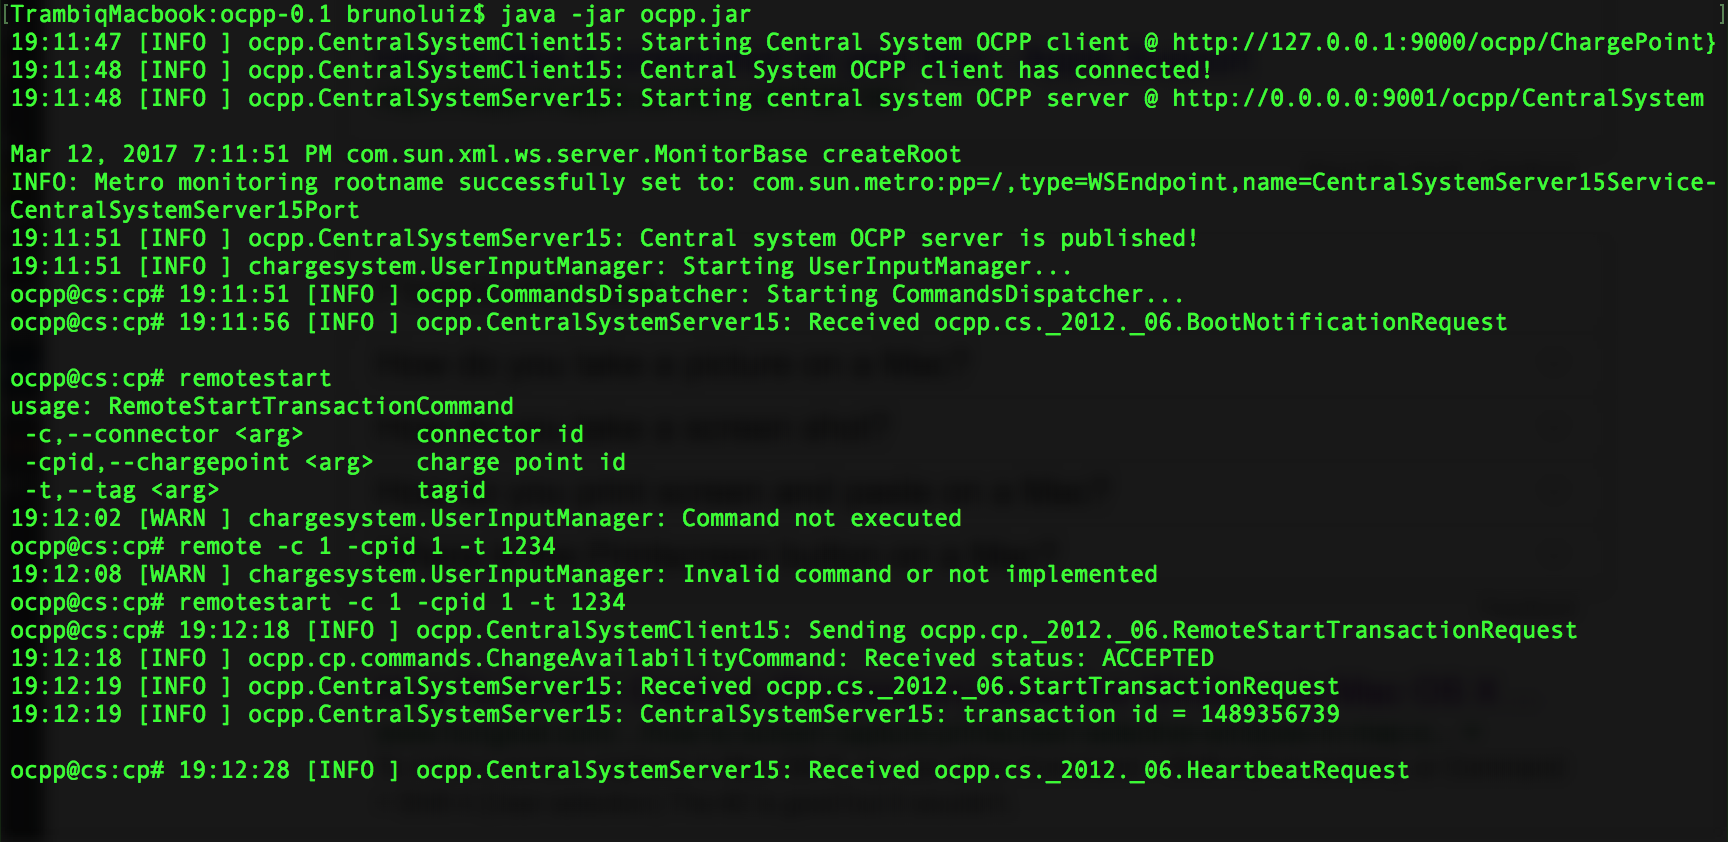
\includegraphics[width=1.0\textwidth,natwidth=2130,natheight=1420,angle=0]{assets/images/ocpp-tool-snap.jpg}
        \caption{Ferramenta que simula servidor OCPP}
        \label{fig:ocpp-tool-snap}
      \end{center}
    \end{figure}

  \section{Implementações e testes iniciais}
  \label{tests:initial}

    O desenvolvimento inicial foi realizado a partir de código fonte existente, no qual não havia implementação funcional da EVSE e apenas possibilitava o teste de cada dispositivo isoladamente. Após essa etapa de revisão de código, iniciou-se a implementação do software da estação.

    Alguns testes unitários foram desenvolvidos sob o \textit{framework} de testes \textit{JUnit}, o que permite o programa ser testado antes de ser embarcado. Após concluir com sucesso a etapa de verificação do software, ou seja, quando os testes unitários não detectam erros, o programa é enviado para a \textit{BeagleBone}. Conforme apresentado na Figura \ref{fig:setup-tests}, a BeagleBone está conectada aos dispositivos listados na seção \ref{methodology:devices}, porém dispostos em uma bancada de testes.

    Como as cargas utilizadas durante o teste consumiam pouca energia (fontes \ac{CA}-\ac{CC} de dispositivos de baixo consumo, como notebooks), o medidor de energia teve seu multiplicador de corrente configurado em 100, possibilitando assim simular um consumo alto de forma rápida (sem precisar aguardar um grande período de tempo para atingir 1 kWh).

    Simulou-se a inicialização e finalização de cargas no conector modo 2, onde foram seguidos fluxos similares as figuras \ref{fig:sw-starttransaction} e \ref{fig:sw-stoptransaction}, já que essas permitem verificar diversos aspectos do sistema: autenticação, comunicação externa e com medidores, criação de transações, verificação de falhas, entre outras.

    O conector modo 3 \textit{Mennekes} não pode ser testado na bancada de testes pois, para habilitar o carregamento, é necessário realizar todo sequenciamento apresentado na figura \ref{fig:phoenix} e este só seria possível se houvesse um veículo próximo a bancada. Portanto, este ficou para ser testado na própria estação protótipo.

    Todos arquivos, incluindo o sistema operacional, são colocados em um cartão SD, o que facilita a cópia desses dados para a realização de cópias de segurança (criação de imagens), possibilitando o intercâmbio do sistema entre a bancada de testes e a estação protótipo.

    \begin{figure}[H]
      \begin{center}
        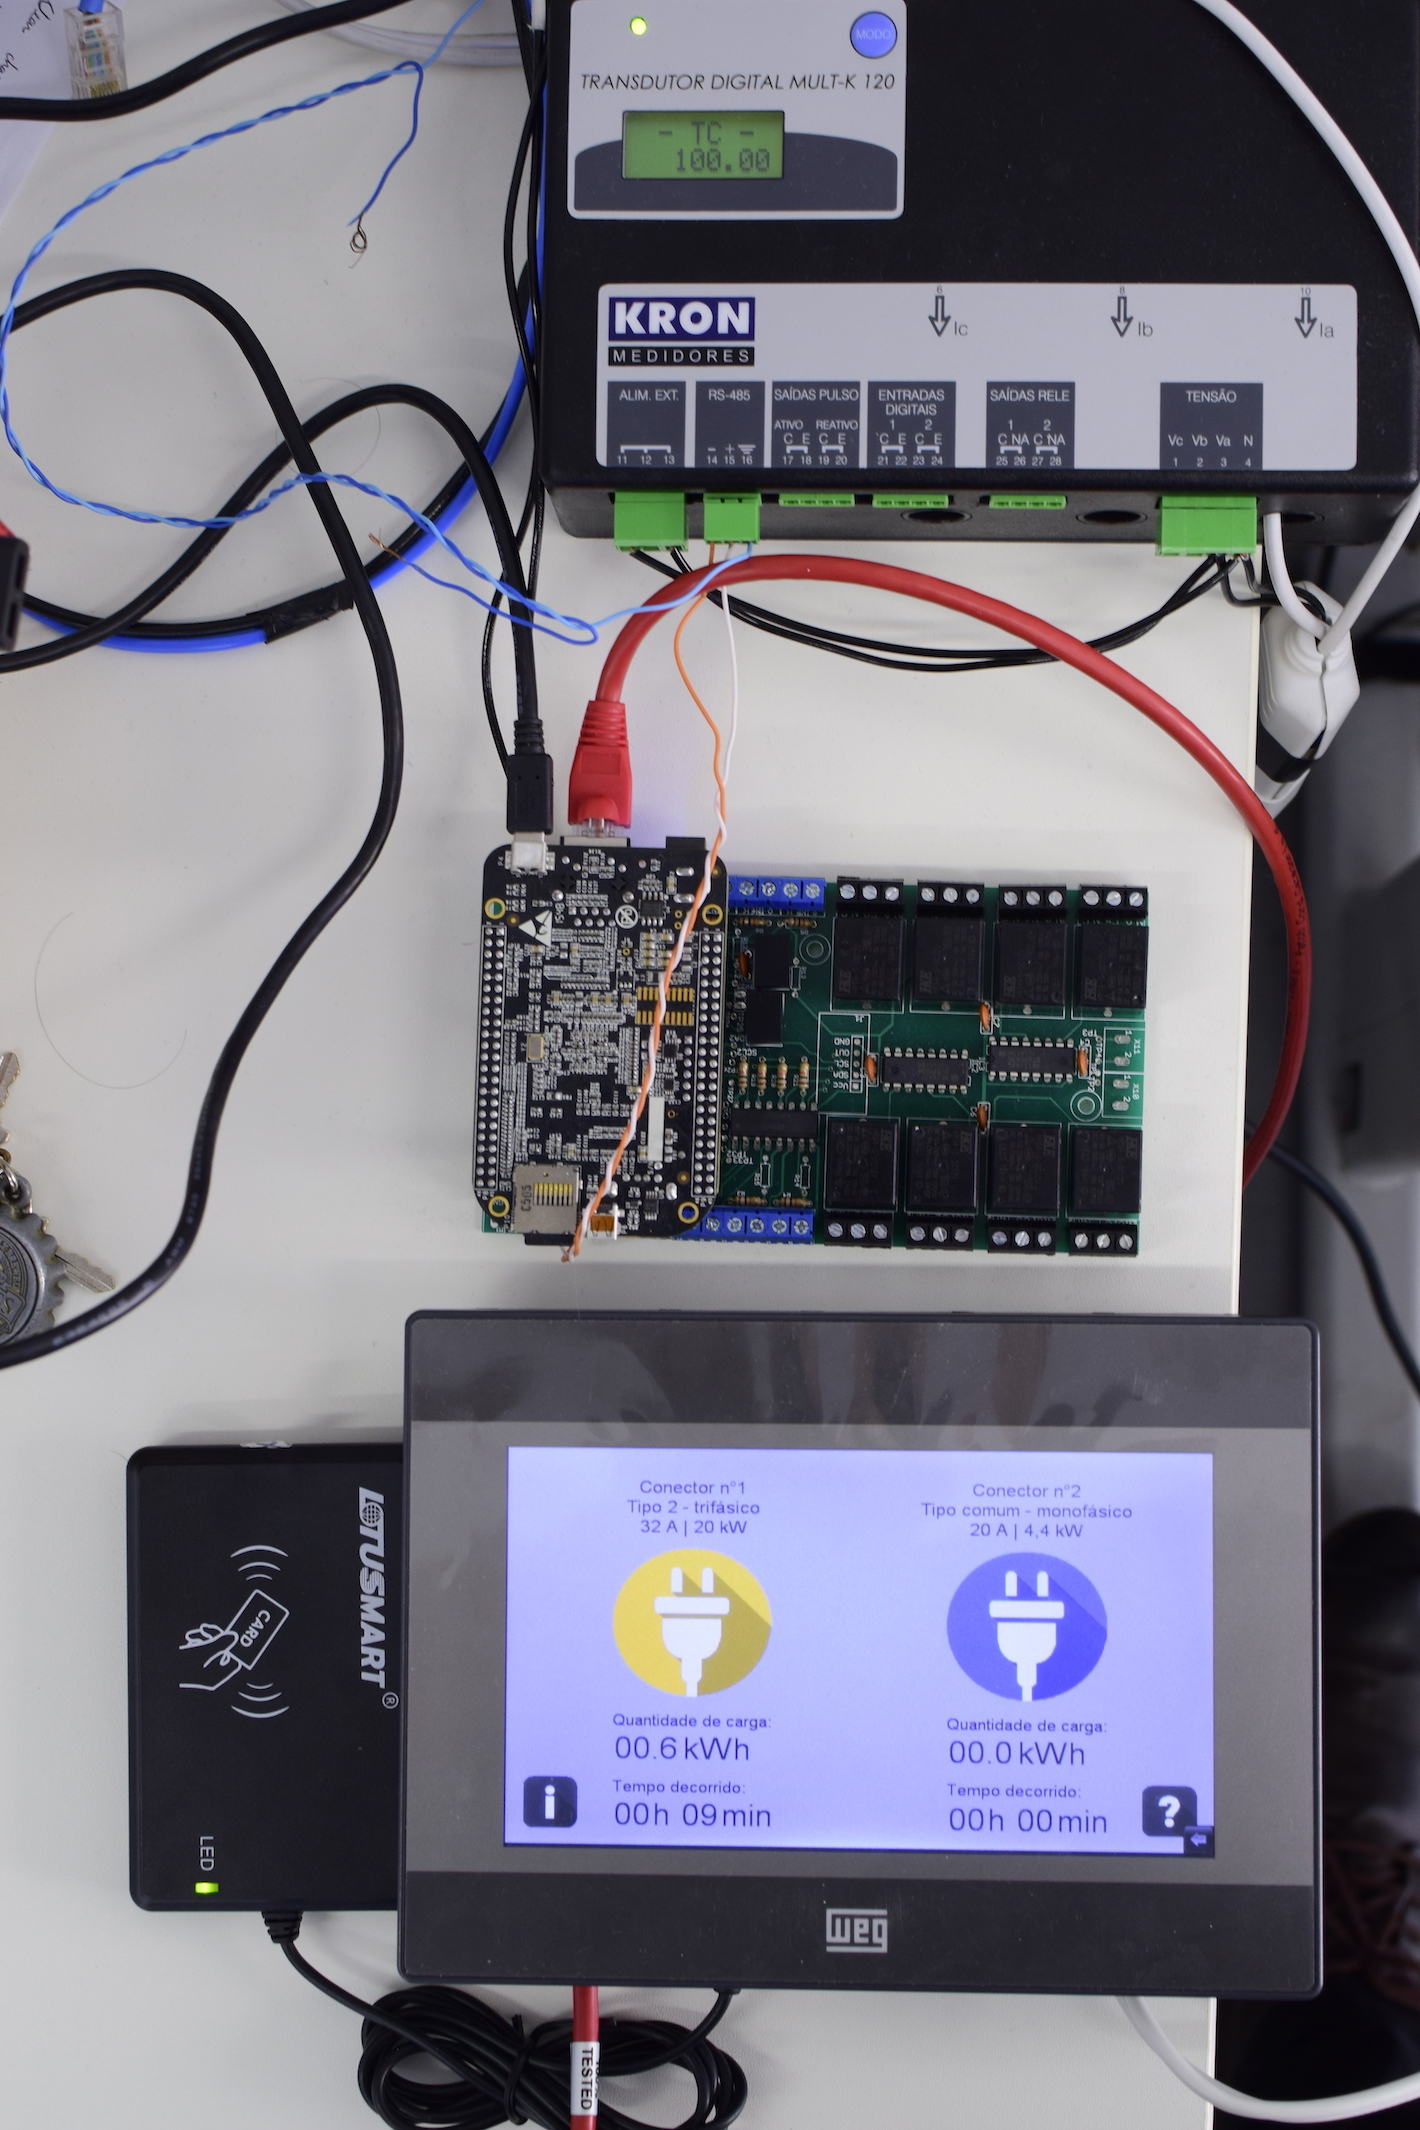
\includegraphics[width=0.6\textwidth,natwidth=2130,natheight=1420,angle=-90]{assets/images/setup-tests.jpg}
        \caption{Disposição dos dispositivos na bancada de testes}
        \label{fig:setup-tests}
      \end{center}
    \end{figure}

  \section{Testes na estação protótipo}
  \label{tests:evse}

    Após executar os testes na bancada, o sistema foi levado para a \textit{\ac{EVSE}} protótipo, situada no estacionamento da Fundação CERTI (figura \ref{fig:evse}). O arranjo dos dispositivos da estação difere da bancada de testes (figura \ref{fig:setup-evse}), porém visto que os dispositivos são os mesmos e o sistema embarcado foi colocado em um cartão SD, só seria necessário inserir o cartão na BeagleBone da estação e configurá-la para realizar a inicialização a partir do cartão, caso já não estiver configurada de fábrica.

    Visto que a estação, no momento da escrita deste projeto, se encontrava sem conectividade, foi utilizado o modo local. Nesse modo, o \textit{software} captura as chamadas que seriam enviadas para o \textit{Central System} e as responde localmente, permitindo seu funcionamento mesmo sem conectividade. 

    \begin{figure}[H]
      \begin{center}
        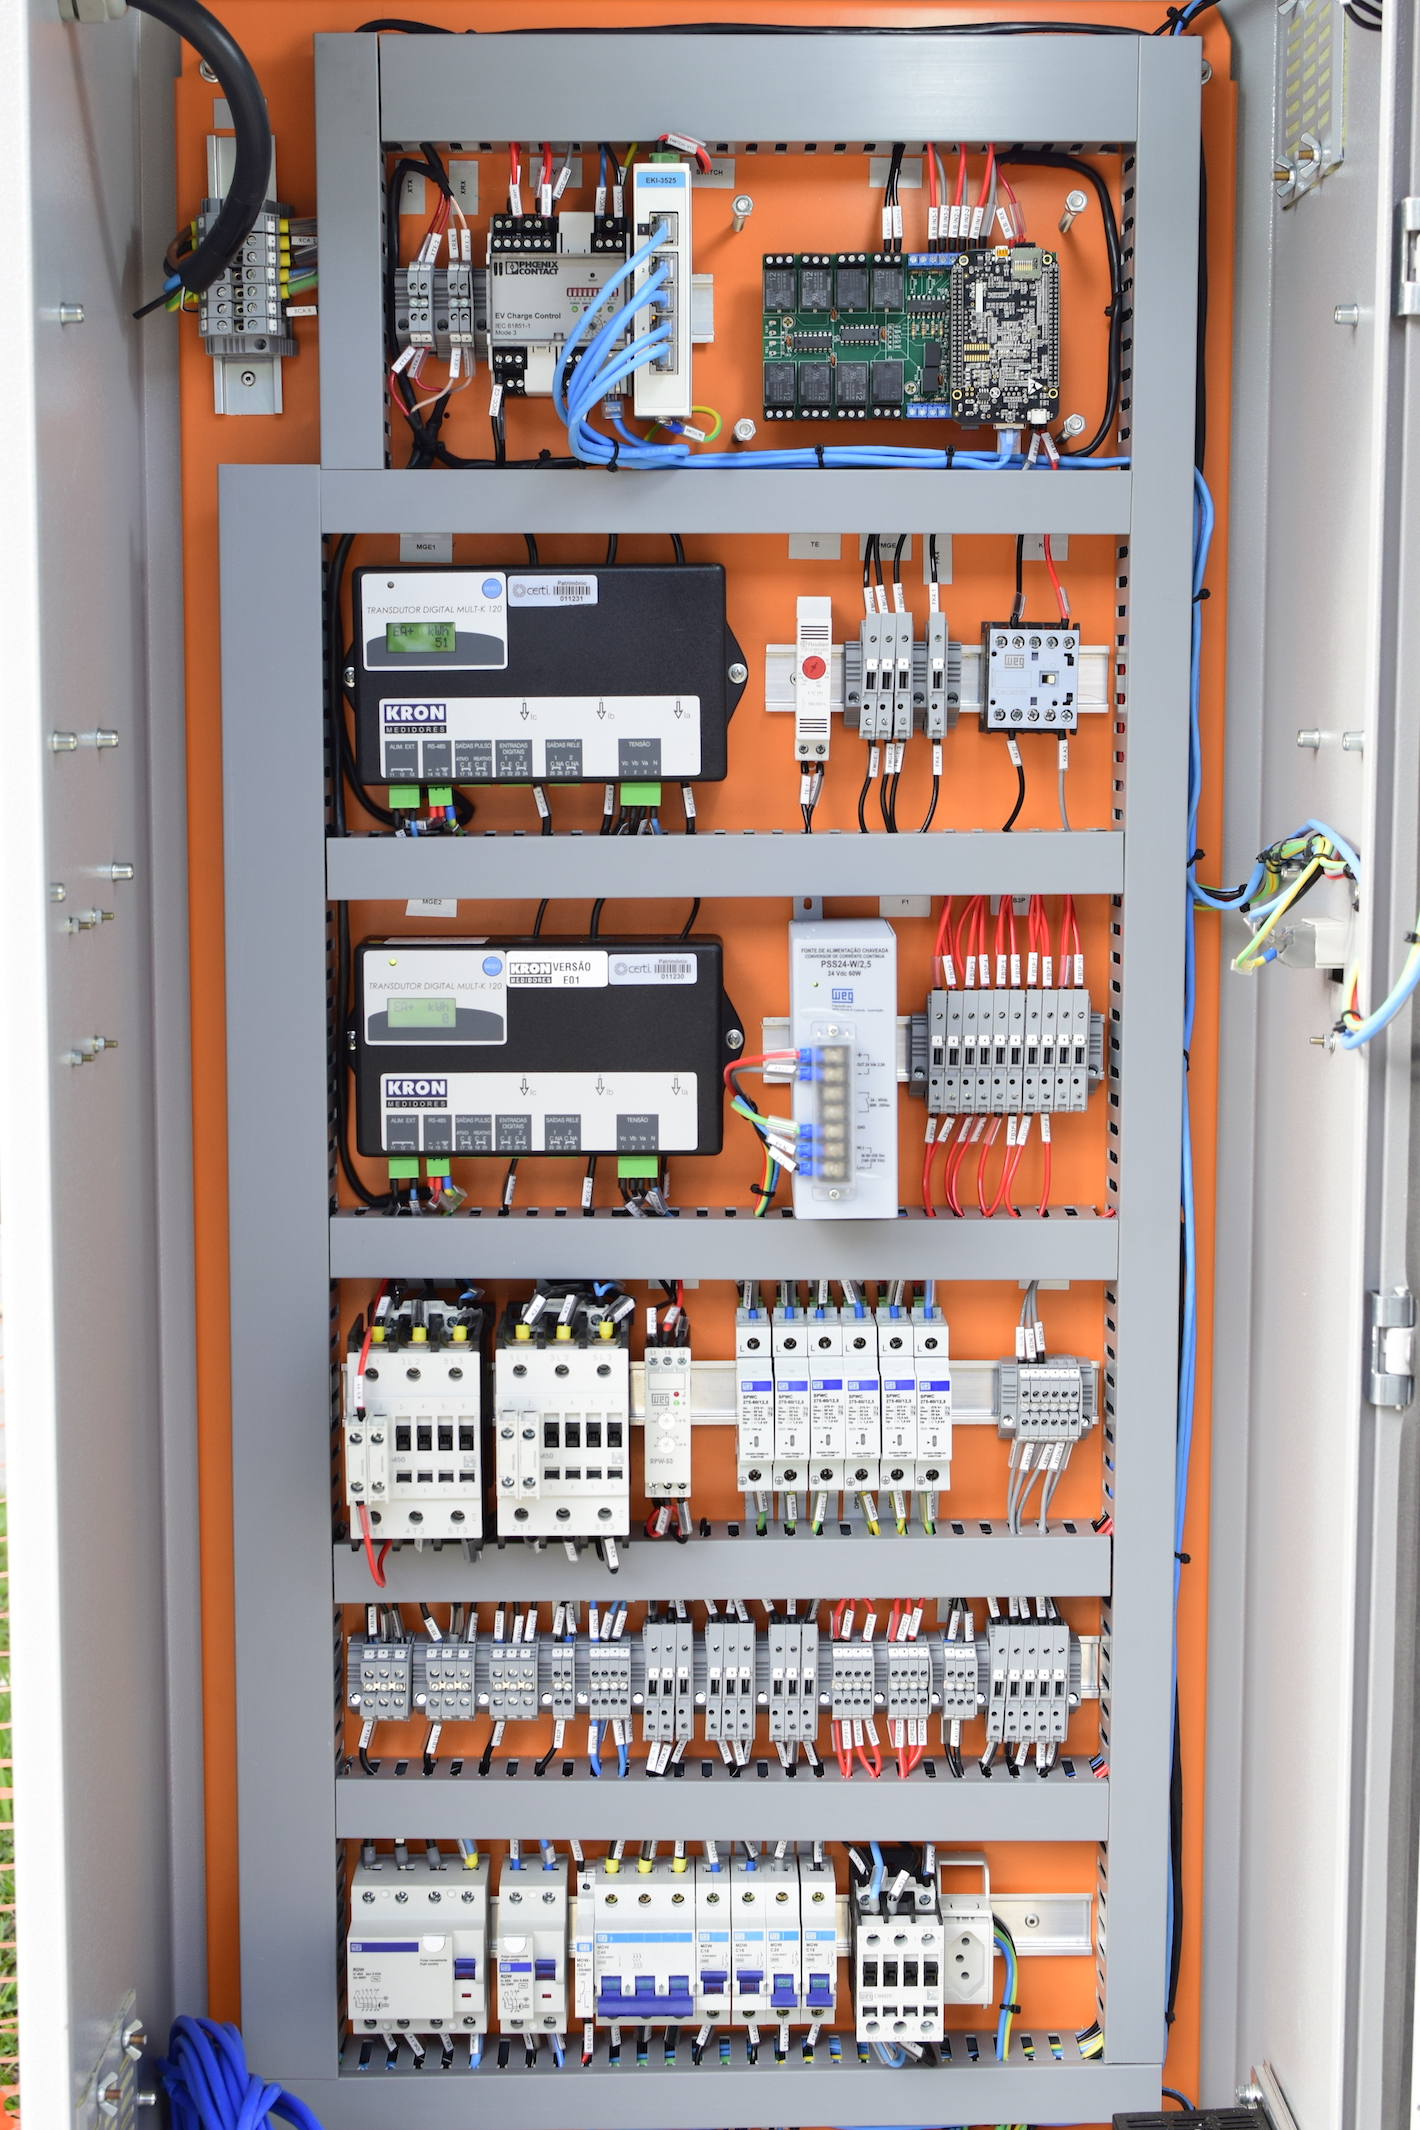
\includegraphics[width=0.5\textwidth,natwidth=1420,natheight=2130]{assets/images/setup-evse.jpg}
        \caption{Disposição dos dispositivos na estação protótipo}
        \label{fig:setup-evse}
      \end{center}
    \end{figure}

    Embora a previsão fosse de que a estação apresentasse o mesmo comportamento da bancada de testes, ao menos para o conector modo 2, não foi isso que ocorreu inicialmente. Um dos problemas observados foi relativo a conectividade da BeagleBone com outros dispositivos Ethernet, que foi resolvido com a substituição do \textit{connman} pelo \textit{Network Manager}. O \textit{connman} possui configurações atreladas a dados únicos de cada dispositivo, o que necessitaria que cada BeagleBone fosse configurada manualmente. Enquanto isso, o \textit{Network Manager} se baseia em configurações fixas no arquivo /etc/network/interfaces, sendo que esse não causou problemas quando executado na estação.

    Outros problemas observados estavam relacionados à comunicação serial: um foi devido as configurações seriais da bancada e da estação serem diferentes, porém isso foi rapidamente detectado e resolvido. Porém, um problema um pouco mais complicado surgiu logo após, quando notamos que o \textit{software} não estava funcionando adequadamente na estação pois não conectava ou perdia leituras. Foi descoberto que alguns circuitos integrados que transformam a saída \textit{\ac{UART}} para RS-485 possuem sua saída conectada a sua entrada, o que acabava gerando problemas na recepção de alguns dados. Após alguns dias foi descoberto que isso se chama \textit{echo} e poderia ser resolvido via \textit{software} (parâmetro \textit{"echo"} da classe de conexão do Jamod).

    \begin{figure}[H]
      \begin{center}
        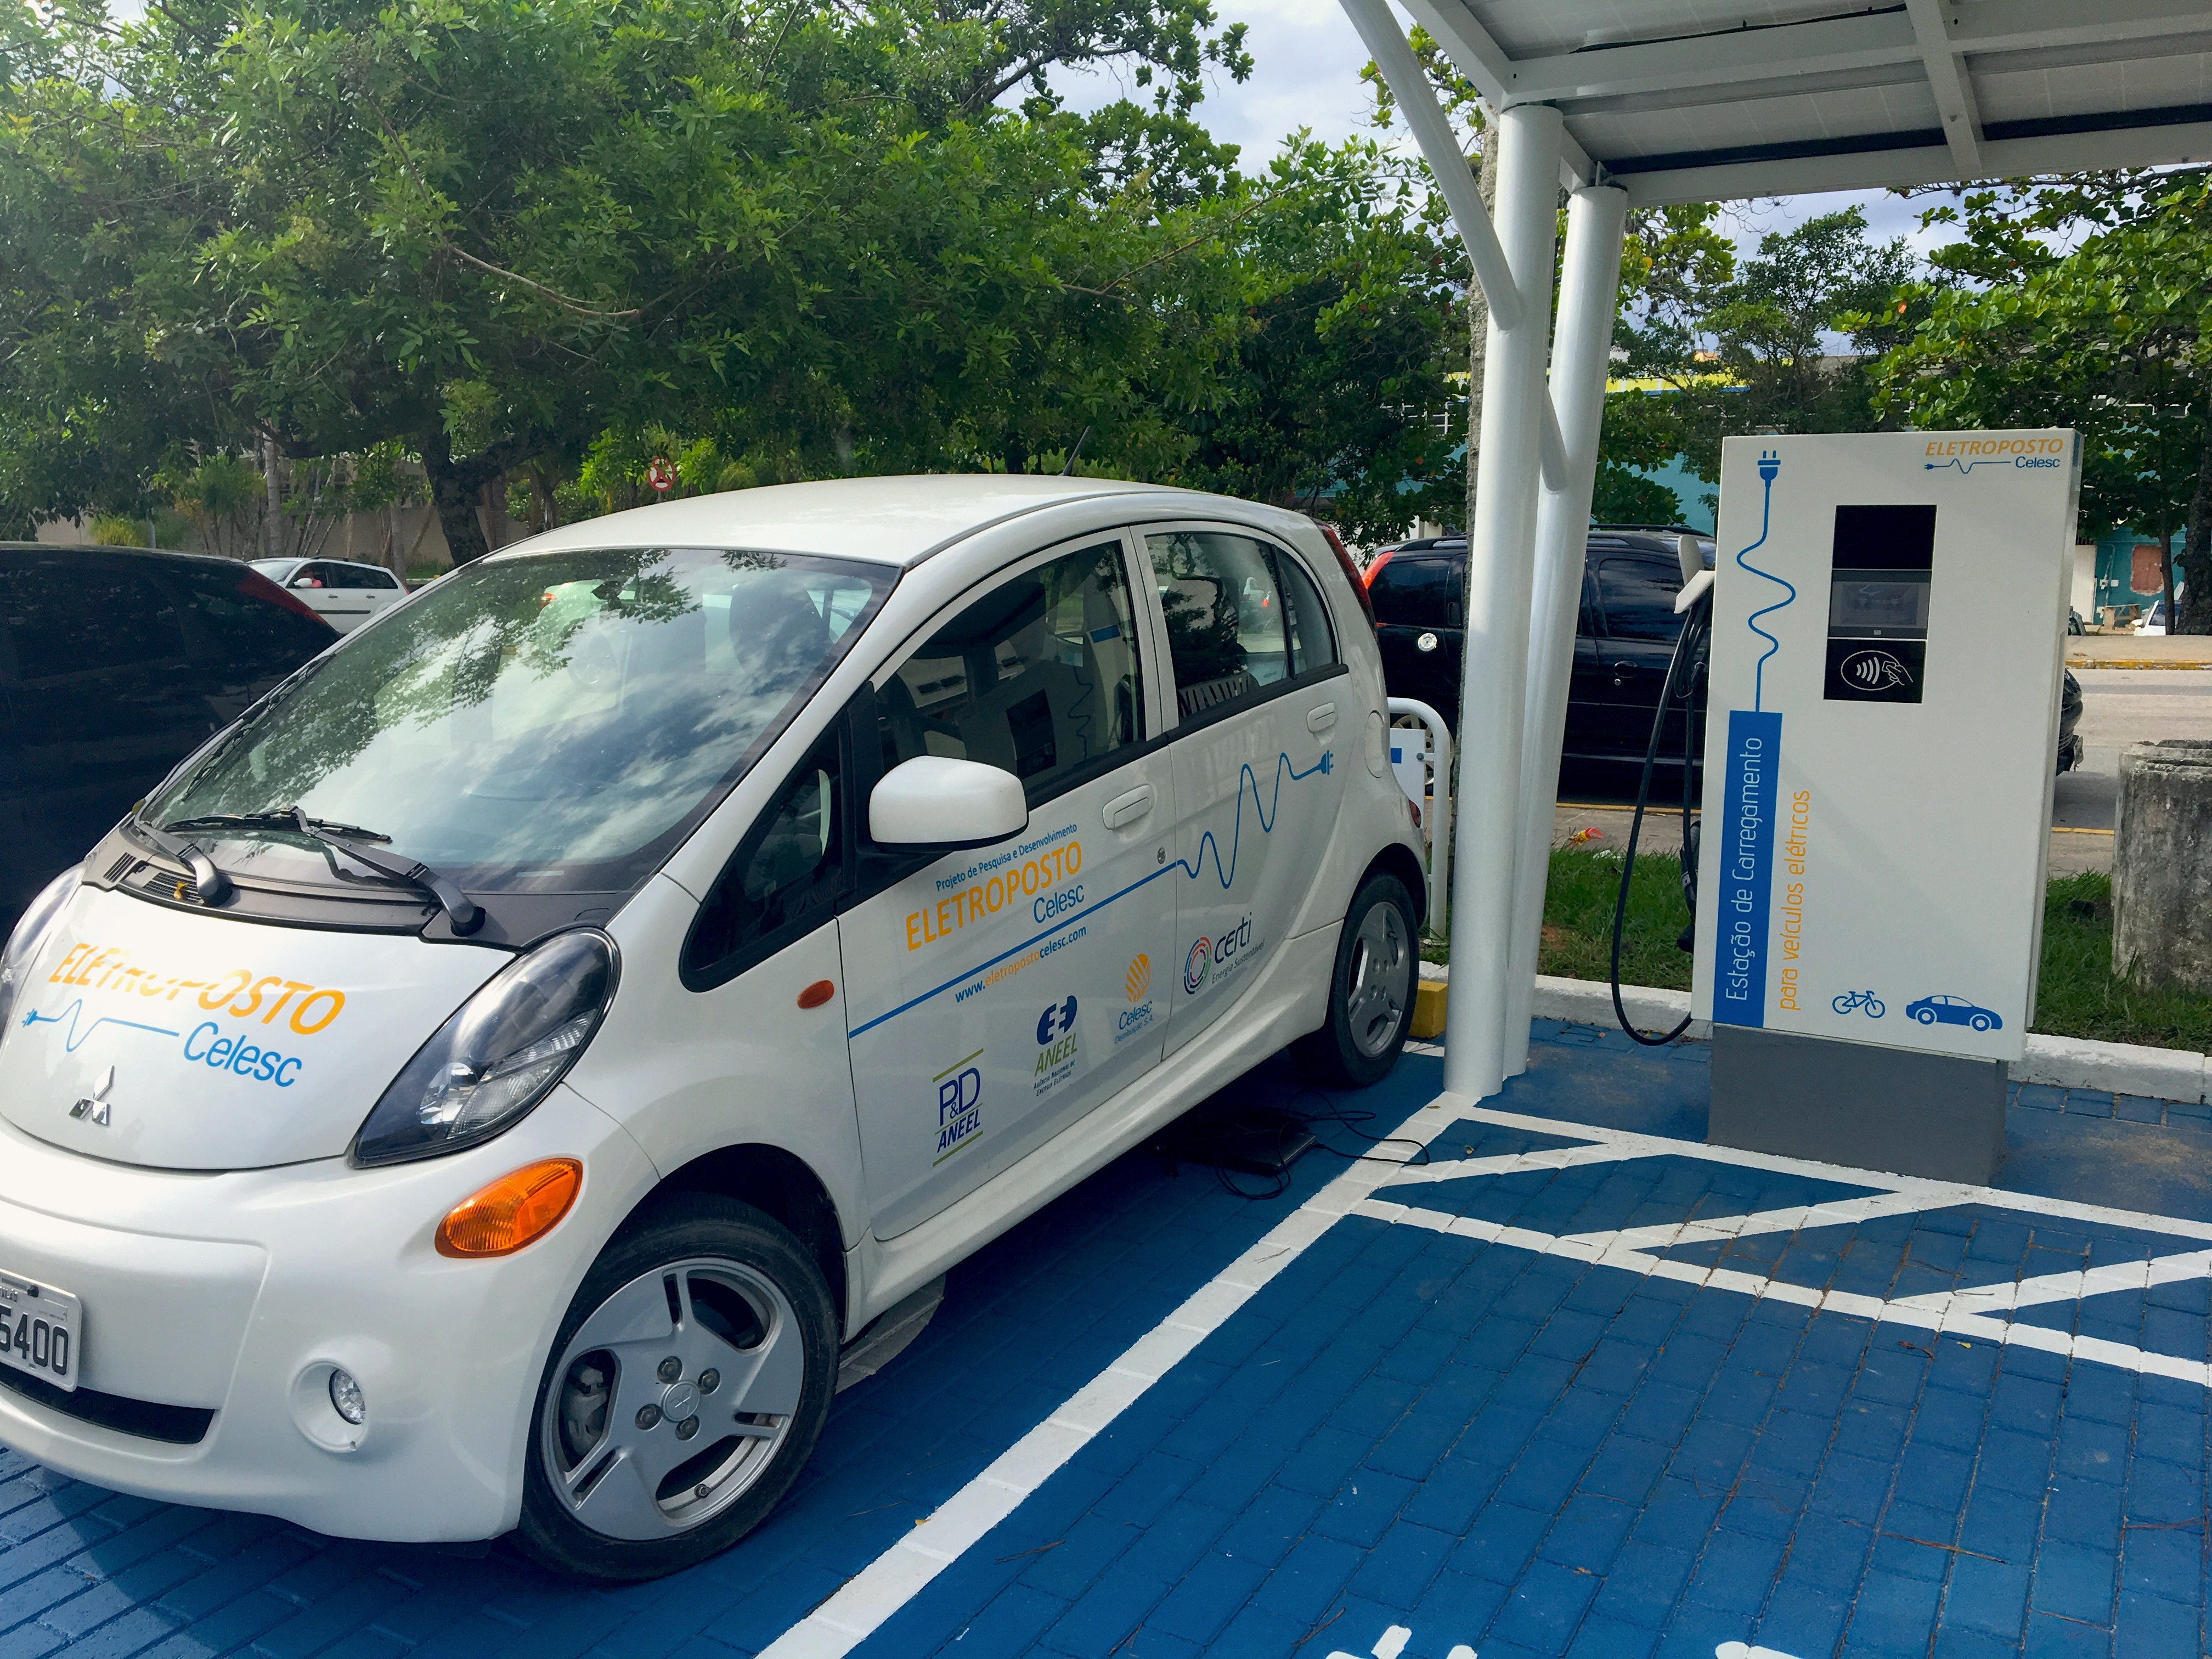
\includegraphics[width=.75\textwidth,natwidth=4032,natheight=3024]{assets/images/evse.jpg}
        \caption{Estação protótipo final com Mitsubishi Miev estacionado}
        \label{fig:evse}
      \end{center}
    \end{figure}

    Como não foi possível testar o conector modo 3 \textit{Mennekes} previamente, alguns problemas surgiram também. O conector do veículo de testes, Mitsubishi Miev, usa o padrão americano. Portanto, é necessário um adaptador para o padrão \textit{Mennekes} para carregá-lo. Porém, tal adaptador gerou falhas elétricas que impossibilitavam o carregamento contínuo do veículo, como mal contato entre os pinos do adaptador e do conector, visto que o \textit{Phoenix} desativa o carregamento imediatamente ao perceber alguma falha. Para resolver esse problema, o adaptador foi cortado em alguns milímetros para possibilitar que os pinos de contato ficassem mais próximos, além de o \textit{software} mandar um comando para o \textit{Phoenix} limitar a corrente máxima permitida (visto que há suspeita de que, devido ao adaptador, o carregamento não pode exigir muita potência). Deste modo foi possível fazer alguns carregamentos experimentais, porém nenhum longo foi realizado devido a limitações de tempo e problemas com o veículo.

    Em um teste anterior com um BMW i3 sem o \textit{software} de controle, foi realizado um carregamento longo, sem nenhuma falha, com o conector \textit{Mennekes}. A figura \ref{fig:evse-charge} mostra a curva de corrente x tempo do carregamento, onde a estação chega a fornecer um máximo de 25,1 A e levou aproximadamente 4h30m para finalizar o carregamento. Poderia ser ainda mais rápido caso a estação possuísse um conector modo 4 (seção \ref{stateofart:modes:europe:mode4}).

    \begin{figure}[H]
      \begin{center}
        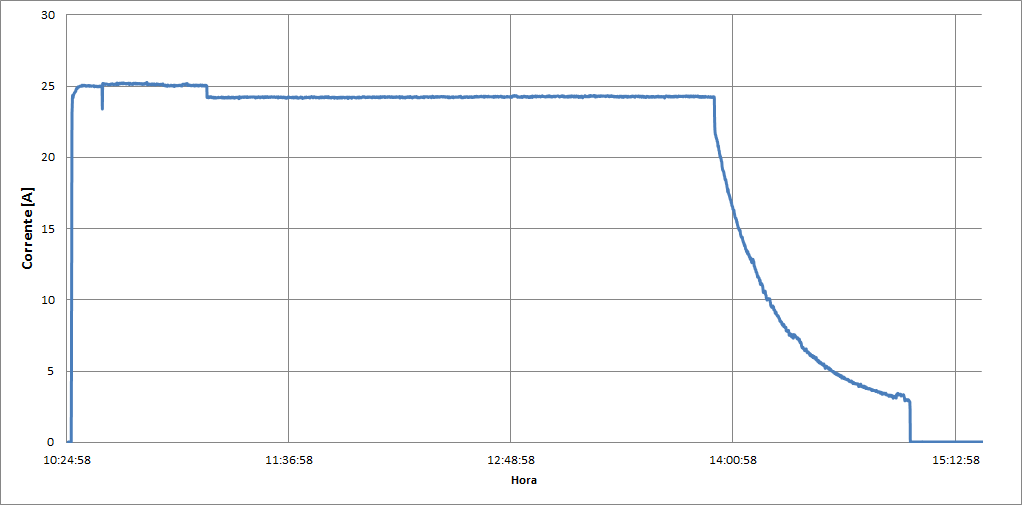
\includegraphics[width=\textwidth,natwidth=1420,natheight=2130]{assets/images/evse-charge.png}
        \caption{Gráfico Corrente x Tempo para carregamento do BMW i3 utilizando o conector modo 3 \textit{Mennekes}}
        \label{fig:evse-charge}
      \end{center}
    \end{figure}

    Foi realizada uma carga de menos de um minuto apenas para mostrar o sequenciamento da estação, visto que o programa gera saídas de texto para diversas operações realizadas internamente e isso permite a visualização do que está ocorrendo na estação. A saída completa está disponível no apêndice \ref{appendix:log}. Nos trechos abaixo, é possível observar o \textit{software} realizar algumas das etapas mostradas nos sequenciamentos das figuras \ref{fig:sw-init}, \ref{fig:sw-starttransaction} e \ref{fig:sw-stoptransaction}.

    \begin{itemize}
      \item Linha 3-23: inicialização do programa 
      \lstinputlisting[basicstyle=\ttfamily\scriptsize]{assets/txt/log1.txt}

      \item Linha 34: usuário utiliza a \textit{\ac{RFID}}
      \lstinputlisting[basicstyle=\ttfamily\scriptsize]{assets/txt/log2.txt}

      \item Linha 35-39: \textit{\ac{RFID}} é autenticada (usuário habilitado para carregamento)
      \lstinputlisting[basicstyle=\ttfamily\scriptsize]{assets/txt/log3.txt}

      \item Linhas 39-41: \textit{software} aguarda usuário selecionar o conector
      \lstinputlisting[basicstyle=\ttfamily\scriptsize]{assets/txt/log4.txt}

      \item Linhas 42-45: inicia a \textit{Thread} da transação e habilita o carregamento
      \lstinputlisting[basicstyle=\ttfamily\scriptsize]{assets/txt/log5.txt}

      \item Linha 46: mostra mensagem para o usuário sobre o início do carregamento
      \lstinputlisting[basicstyle=\ttfamily\scriptsize]{assets/txt/log6.txt}

      \item Linhas 48-54: notifica servidor \textit{\ac{OCPP}} sobre o início do carregamento
      \lstinputlisting[basicstyle=\ttfamily\scriptsize]{assets/txt/log7.txt}

      \item Linhas 55-86: \textit{software} envia dados para servidor e alterna entre algumas telas na \ac{IHM}
      \lstinputlisting[basicstyle=\ttfamily\scriptsize]{assets/txt/log8.txt}

      \item Linhas 87-88: carregamento cancelado devido desconexão do veículo por parte do usuário
      \lstinputlisting[basicstyle=\ttfamily\scriptsize]{assets/txt/log9.txt}

      \item Linhas 89-95: notifica servidor \textit{\ac{OCPP}} sobre o término do carregamento
      \lstinputlisting[basicstyle=\ttfamily\scriptsize]{assets/txt/log10.txt}
    \end{itemize}